% pentagon-perturb.tex — \input'd from experiments/experiments.tex
%
% Perturbation study of the HK-O pentagon counterexample.
%
% Sources:
%   - Generated data: experiments/data/pentagon-perturb.jsonl
%   - Plot script: experiments/scripts/pentagon_perturb.py
%   - Experiment notes: experiments/scripts/pentagon_perturb.md
%
% Structure:
%   - Perturbation setup
%   - Histogram of systolic ratios
%   - Summary stats and PCA table

\subsection{HK-O Pentagon Perturbations}
\label{sec:pentagon-perturb}

We perturb the standard HK-O pentagon counterexample by adding small uniform
noise to each facet normal component and each height, renormalizing each
normal to unit length. We generate 100 perturbed samples and compute
$c_{\mathrm{EHZ}}$ using the HK2017 pruned algorithm. This probes the local
stability of the counterexample under small geometric perturbations.

Figure~\ref{fig:pentagon-perturb-hist} shows the histogram of systolic ratios
$\mathrm{sys} = c_{\mathrm{EHZ}}^2/(2\,\mathrm{vol})$ for the perturbed samples,
with the unperturbed value marked for reference.
All perturbed samples fall in the interval between $1$ and the unperturbed value, indicating that the counterexample is a local maximum of the systolic ratio in the perturbation space.
This may not mean that the counterexample is a local maximum among all polytopes with regards to Hausdorff distance, since we only considered perturbations that preserve the facet count $F=10$.

\begin{figure}[h]
\centering
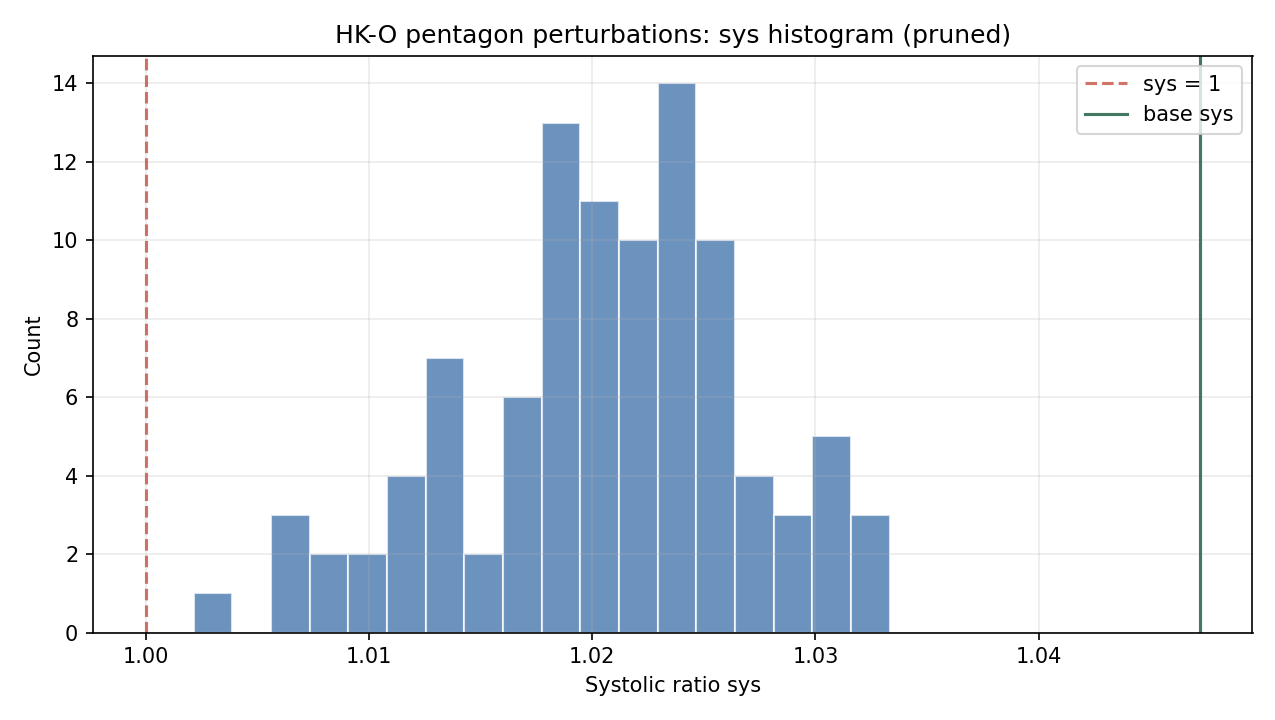
\includegraphics[width=0.9\textwidth]{../experiments/pentagon-perturb/pentagon_perturb_sys_hist.png}
\caption{HK-O pentagon perturbations: systolic ratio histogram for 100 perturbed
  samples. The dashed line marks $\mathrm{sys}=1$, and the solid line marks the
  unperturbed counterexample.}
\label{fig:pentagon-perturb-hist}
\end{figure}

\begin{table}[h]
\centering
\begin{tabular}{rrrrrrr}
\toprule
$N$ & Mean & Median & Std & Min & Max & Base sys \\
\midrule
100 & 1.0287 & 1.0298 & 0.0048 & 1.0142 & 1.0385 & 1.0472 \\
\bottomrule
\end{tabular}
\caption{HK-O pentagon perturbations: summary statistics for the perturbed systolic ratios.}
\label{tab:pentagon-perturb-stats}
\end{table}


%We also compute PCA on the 50D perturbation vectors
%$(\Delta n, \Delta h) \in \mathbb{R}^5$ for each of the 10 facets, using only
%perturbed samples and centering the data. Table~\ref{tab:pentagon-perturb-pca}
%reports the base polytope row and the top PCA components, with the last column
%showing the explained variance ratio.

%\begin{table}[p]
\centering
\scriptsize
\setlength{\tabcolsep}{2pt}
\renewcommand{\arraystretch}{1.1}
\begin{tabular}{lccccccccccc}
\toprule
 Component & Facet 1 & Facet 2 & Facet 3 & Facet 4 & Facet 5 & Facet 6 & Facet 7 & Facet 8 & Facet 9 & Facet 10 & Strength \\
\midrule
 base & (0.8090, 0.5878, 0.0000, 0.0000; 0.8090) & (-0.3090, 0.9511, 0.0000, 0.0000; 0.8090) & (-1.0000, 0.0000, 0.0000, 0.0000; 0.8090) & (-0.3090, -0.9511, 0.0000, 0.0000; 0.8090) & (0.8090, -0.5878, 0.0000, 0.0000; 0.8090) & (0.0000, 0.0000, 0.5878, -0.8090; 0.8090) & (0.0000, 0.0000, 0.9511, 0.3090; 0.8090) & (0.0000, 0.0000, 0.0000, 1.0000; 0.8090) & (0.0000, 0.0000, -0.9511, 0.3090; 0.8090) & (0.0000, 0.0000, -0.5878, -0.8090; 0.8090) & 1.0472 \\
 PC1 & (-0.0218, 0.0294, 0.1102, 0.1372; 0.1445) & (-0.1134, -0.0377, 0.0173, -0.1247; -0.1665) & (-0.0000, 0.2067, 0.0497, -0.1798; 0.2031) & (0.2079, -0.0676, 0.2247, 0.3747; -0.0339) & (0.0718, 0.0986, -0.0185, -0.0322; -0.1337) & (0.2742, 0.1497, -0.1171, -0.0852; -0.1525) & (-0.0398, 0.0013, -0.0209, 0.0636; 0.2037) & (0.0990, 0.0760, 0.1489, -0.0005; 0.3033) & (-0.0430, -0.0799, 0.0648, 0.1996; -0.1010) & (0.0933, -0.2849, 0.0941, -0.0683; -0.1064) & 0.0595 \\
 PC2 & (0.0314, -0.0429, 0.2109, -0.2038; 0.2905) & (0.1219, 0.0392, -0.0983, -0.0012; 0.0142) & (-0.0003, -0.0127, 0.0184, -0.2439; -0.1141) & (-0.1088, 0.0359, 0.0528, 0.1478; 0.0536) & (-0.1012, -0.1386, 0.3548, 0.0852; -0.1435) & (-0.1337, 0.0078, 0.1171, 0.0849; -0.3191) & (-0.2727, 0.1341, 0.0237, -0.0724; 0.2231) & (-0.0674, 0.1738, -0.1848, 0.0002; -0.2006) & (0.2100, -0.0102, -0.0091, -0.0266; 0.0393) & (-0.1615, 0.0689, 0.0953, -0.0690; -0.1217) & 0.0559 \\
 PC3 & (-0.0804, 0.1101, 0.2901, 0.2153; 0.1526) & (0.2404, 0.0778, 0.1173, -0.1379; 0.1310) & (0.0006, -0.0927, -0.0505, -0.0959; 0.1525) & (0.1759, -0.0572, -0.0554, 0.1114; -0.1335) & (0.1525, 0.2098, 0.1476, 0.0883; 0.0847) & (-0.2944, -0.0369, 0.0073, 0.0055; -0.0273) & (0.1146, -0.0144, 0.0043, -0.0140; -0.0075) & (0.1070, -0.0776, -0.2083, -0.0004; -0.1081) & (-0.3244, -0.2313, -0.0114, -0.0350; -0.1716) & (-0.0084, 0.0329, -0.1310, 0.0953; 0.3267) & 0.0543 \\
 PC4 & (0.0017, -0.0014, 0.0365, -0.1675; -0.0080) & (-0.0398, -0.0130, 0.0090, -0.1222; 0.1731) & (-0.0004, 0.1029, 0.1721, -0.0695; 0.2441) & (-0.0709, 0.0228, -0.0334, 0.1706; 0.1753) & (0.0314, 0.0433, -0.1583, -0.4055; -0.0840) & (0.0848, 0.1323, -0.1409, -0.1030; 0.2413) & (-0.0245, -0.0337, 0.0595, -0.1838; 0.0475) & (0.1795, -0.1895, -0.1573, -0.0002; -0.1902) & (0.1655, 0.0661, 0.0015, 0.0034; -0.3110) & (-0.2435, 0.2853, -0.0021, 0.0021; -0.0169) & 0.0527 \\
 PC5 & (-0.1684, 0.2325, -0.1661, 0.1090; 0.2137) & (-0.2172, -0.0707, 0.1600, -0.2003; 0.2480) & (0.0001, 0.2759, -0.0766, 0.0434; -0.2196) & (-0.1636, 0.0528, 0.1097, 0.0195; 0.1170) & (-0.0212, -0.0292, -0.1012, 0.1087; -0.0766) & (-0.0822, -0.0240, -0.2029, -0.1470; 0.0474) & (0.1671, -0.0589, -0.0552, 0.1694; -0.0727) & (-0.2158, 0.3400, -0.1930, 0.0001; 0.0677) & (0.0951, -0.2016, -0.0413, -0.1264; -0.0504) & (-0.1400, 0.0337, -0.0042, 0.0031; 0.0256) & 0.0500 \\
\bottomrule
\end{tabular}
\caption{HK-O pentagon perturbations: PCA components of the 50D perturbation space, listed per facet as $(\Delta n, \Delta h) \in \mathbb{R}^5$. The last column shows explained variance ratio for each component, and the base row reports the unperturbed systolic ratio.}
\label{tab:pentagon-perturb-pca}
\end{table}

